%%%%%%%%%%%%%%%%%%%%%%%%%%%%%%%%%%%%%%%%%
% Beamer Presentation
% LaTeX Template
% Version 1.0 (10/11/12)
%
% This template has been downloaded from:
% http://www.LaTeXTemplates.com
%
% License:
% CC BY-NC-SA 3.0 (http://creativecommons.org/licenses/by-nc-sa/3.0/)
%
%%%%%%%%%%%%%%%%%%%%%%%%%%%%%%%%%%%%%%%%%

%----------------------------------------------------------------------------------------
%	PACKAGES AND THEMES
%----------------------------------------------------------------------------------------

\documentclass{beamer}

\mode<presentation> {

% The Beamer class comes with a number of default slide themes
% which change the colors and layouts of slides. Below this is a list
% of all the themes, uncomment each in turn to see what they look like.

%\usetheme{default}
%\usetheme{AnnArbor}
%\usetheme{Antibes}
%\usetheme{Bergen}
%\usetheme{Berkeley}
%\usetheme{Berlin}
%\usetheme{Boadilla}
%\usetheme{CambridgeUS}
%\usetheme{Copenhagen}
%\usetheme{Darmstadt}
%\usetheme{Dresden}
%\usetheme{Frankfurt}
%\usetheme{Goettingen}
%\usetheme{Hannover}
%\usetheme{Ilmenau}
%\usetheme{JuanLesPins}
%\usetheme{Luebeck}
\usetheme{Madrid}
%\usetheme{Malmoe}
%\usetheme{Marburg}
%\usetheme{Montpellier}
%\usetheme{PaloAlto}
%\usetheme{Pittsburgh}
%\usetheme{Rochester}
%\usetheme{Singapore}
%\usetheme{Szeged}
%\usetheme{Warsaw}

% As well as themes, the Beamer class has a number of color themes
% for any slide theme. Uncomment each of these in turn to see how it
% changes the colors of your current slide theme.

%\usecolortheme{albatross}
%\usecolortheme{beaver}
%\usecolortheme{beetle}
%\usecolortheme{crane}
%\usecolortheme{dolphin}
%\usecolortheme{dove}
%\usecolortheme{fly}
%\usecolortheme{lily}
%\usecolortheme{orchid}
%\usecolortheme{rose}
%\usecolortheme{seagull}
%\usecolortheme{seahorse}
%\usecolortheme{whale}
%\usecolortheme{wolverine}

%\setbeamertemplate{footline} % To remove the footer line in all slides uncomment this line
%\setbeamertemplate{footline}[page number] % To replace the footer line in all slides with a simple slide count uncomment this line

%\setbeamertemplate{navigation symbols}{} % To remove the navigation symbols from the bottom of all slides uncomment this line
}

\usepackage{graphicx} % Allows including images
\usepackage{booktabs} % Allows the use of \toprule, \midrule and \bottomrule in tables
\usepackage{multirow}
\newcommand{\xmark}{\textcolor{red}{\text{\sffamily X}}}
\newcommand{\cmark}{\textcolor{green}{\checkmark}}
\newcommand{\tr}{\text{tr}}
\newcommand{\E}{\textbf{E}}
\newcommand{\diag}{\text{diag}}
\newcommand{\argmax}{\text{argmax}}
\newcommand{\argmin}{\text{argmin}}
\newcommand{\Cov}{\text{Cov}}
\newcommand{\Vol}{\text{Vol}}

%----------------------------------------------------------------------------------------
%	TITLE PAGE
%----------------------------------------------------------------------------------------


\title{A practical evaluation of recent methods in high-dimensional inference}

\author{Charles Zheng} % Your name
\institute[Stanford] % Your institution as it will appear on the bottom of every slide, may be shorthand to save space
{Stanford University}
\date{\today} % Date, can be changed to a custom date

\begin{document}

\begin{frame}
\titlepage % Print the title page as the first slide
\end{frame}

\section{Introduction}

\begin{frame}
\frametitle{Problem and motivation}
\begin{itemize}
\item $x \in \mathbb{R}^p, y \in \mathbb{R}$ have a joint distribution $P$ where $y|x \sim N(x^T \beta, \sigma^2)$
\item Observe $X = (x_1, \hdots, x_n)^T$, $Y = (y_1,\hdots, y_n)$ iid
\item Problem: test $H_i: \beta_0 = i$ for $i = 1,\hdots, p$
\item Motivation: $x$ are SNPs (mutations), $y$ is phenotype
\end{itemize}
\end{frame}

\begin{frame}
\frametitle{Methods}
\begin{center}
\begin{tabular}{|c|c|c|} \hline
 & Control & $p > n$\\ \hline
Classical inference (Pearson 1930) & Marginal & No \\ \hline
Debiased lasso (Javanmard et al. 2014) & Marginal & Yes\\ \hline
Knockoffs (Barber et al. 2014) & FDR & ? \\ \hline
Covariance test (Lockhart et al. 2014) &  ?? & Yes \\ 
... + FDR control (G'Sell et al. 2013) &  FDR & Yes \\ \hline
 & &  \\ \hline
\end{tabular}
\end{center}
\end{frame}

\begin{frame}
\frametitle{The LASSO path}
All three methods share an association with LASSO:
\[
\hat{\beta}_\lambda = \text{argmin}_\beta \frac{1}{2}||X\beta - Y||^2 + \lambda ||\beta||_1
\]
\begin{center}
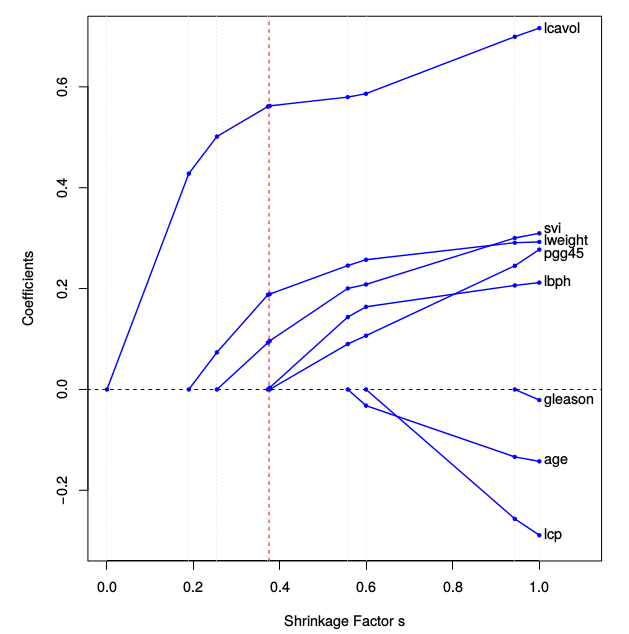
\includegraphics[scale = 0.25]{lasso_path.png}
\end{center}
\emph{(Image credit: ??)}
\end{frame}

\begin{frame}
\frametitle{Debiased regularized M-estimators}
\begin{itemize}
\item (2014) Javanmard and Montanari
\item Standard assumptions + sparsity condition on $\beta$ + large $n$ and $p$ asymptotics
\end{itemize}
\begin{center}
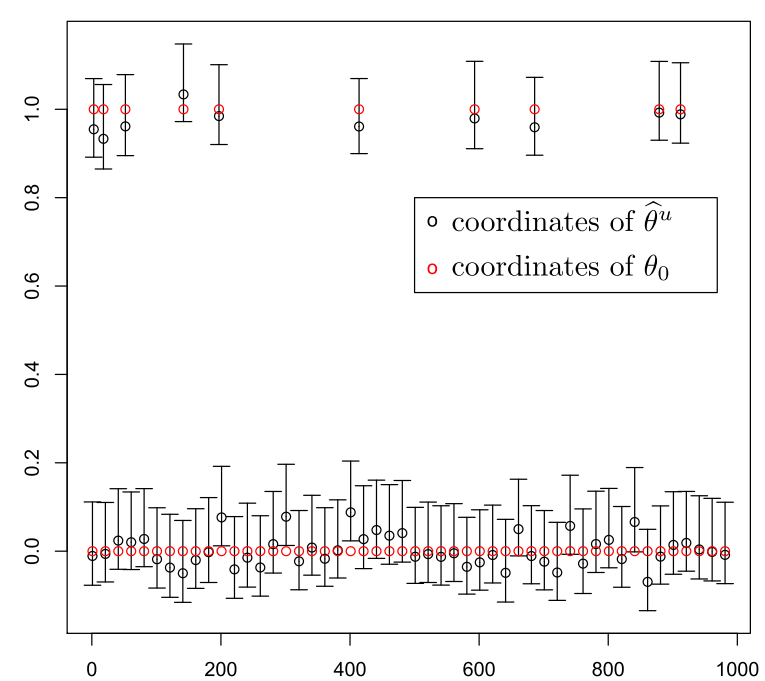
\includegraphics[scale = 0.25]{javanmard.png}
\end{center}
\end{frame}

\begin{frame}
\frametitle{Knockoff filter}
\begin{itemize}
\item (2014) Barber and Cand\'{e}s
\item \emph{Finite sample} $Y \sim N(X\beta, \sigma^2 I)$, $n \leq p$, control FDR
\item Extension to $p > n$, FWER control, etc. forthcoming...
\end{itemize}
\begin{center}
\begin{tabular}{cc}
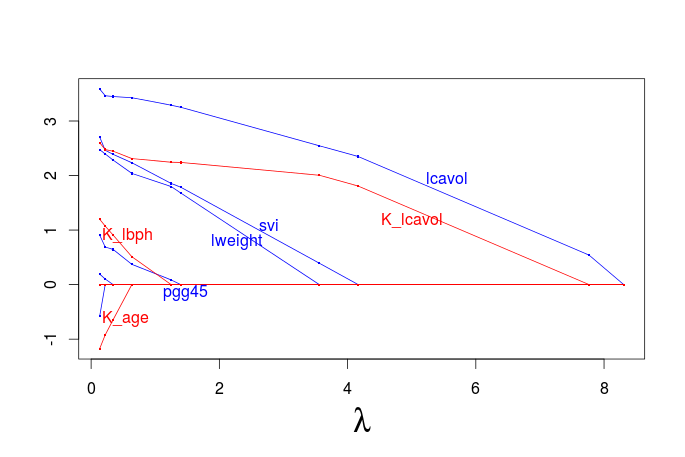
\includegraphics[scale = 0.25]{knockoff.png} &
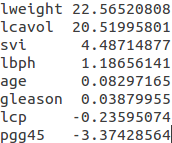
\includegraphics[scale = 0.5, trim=0in -1in 0.5in 0in, clip]{knockoff2.png}
\end{tabular}
\end{center}
\end{frame}

\begin{frame}
\frametitle{Covariance test}
\begin{itemize}
\item (2014) Lockhart, Taylor, Tibshirani (x 2)
\item Standard assumptions $Y \sim N(X\beta, \sigma^2 I)$ + large $p$ asymptotics
\item \emph{See also} non-asymptotic exact test (Lee, Sun x 2, Taylor 2015)
\item What kind of Type I error does it control?
\end{itemize}
\begin{center}
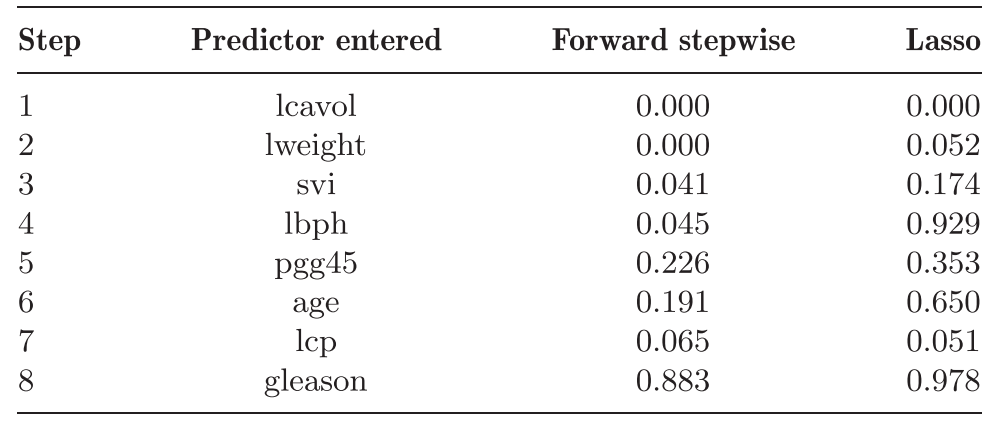
\includegraphics[scale = 0.25]{covtest.png}
\end{center}
\end{frame}

\begin{frame}
\frametitle{FDR control for covariance test}
\begin{itemize}
\item G'Sell, Wager, Chouldechova, Tibshirani (2013)
\item Two methods to control FDR for convariance test... but under a \emph{different} definition of Type I error
\end{itemize}
\end{frame}

\begin{frame}
\frametitle{Formulations for hypothesis testing}
\begin{itemize}
\item<1-5> For a subset $E$ of the variables, define $\beta^E = (X_E^T X_E)^{-1} X_E^T X\beta$
\item<2-> \textbf{The full model null}.  Test multiple hypotheses $H_i: \beta_i = 0$
\item<6> In this talk, we define type I errors according to \emph{full model
  null}... 
\item<3> \textbf{Selective inference}.  Condition on a randomly selected subset $E$, test hypotheses $H_i: \beta^E_i = 0$ for all $i \in E$
\item<4-5> \textbf{Incremental null}.  (Informal explanation).  I make
  a mistake whenever I add a variable to the model which
  \emph{doesn't} improve the fit of the model.
\item<5> FDR control for covariance test controls for the
  \emph{incremental null}.  That is, out of the variables I reject, I
  control the number of variables \emph{which were redundant} at the
  time I added them.  However, if a variable is initially useful and
  only becomes redundant as more variables are added, it is not
  considered a mistake.
\end{itemize}
\end{frame}


\begin{frame}
\frametitle{Methods}
But what's actually used in practice?
\begin{center}
\begin{tabular}{|c|c|c|} \hline
 & Control & $p > n$\\ \hline
Classical inference (Pearson 1930) & Marginal & No \\ \hline
Debiased lasso (Javanmard et al. 2014) & Marginal & Yes\\ \hline
Knockoffs (Barber et al. 2014) & FDR & ? \\ \hline
Covariance test (Lockhart et al. 2014) &  ?? & Yes \\
... + FDR control (G'Sell et al. 2013) &  FDR & Yes \\ \hline
\textbf{Marginal screening} & ??? & Yes \\ \hline
\end{tabular}
\end{center}
\end{frame}

\begin{frame}
\frametitle{Regression vs Marginal Screening}
Testing $H_i: \beta_i = 0$ is better than testing $H_i: \Cov(X_i, Y) = 0$
when you are looking for $X_i$ \emph{directly} linked to $Y$
\begin{center}
\begin{tabular}{cc}
\multirow{5}{*}{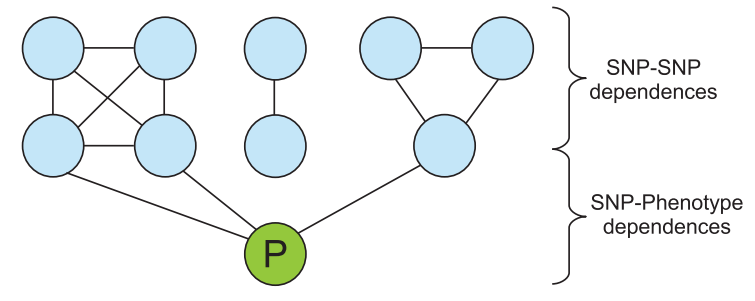
\includegraphics[scale = 0.3]{pgm.png}} & \\
& $\beta_i = 0$\\
& \vspace{0.2in}\\
& $\beta_i \neq 0$\\
& \vspace{0.2in}\\
\end{tabular}
\end{center}
(Adapted from \emph{Mourad 2012})
\end{frame}

\begin{frame}
\frametitle{Statistical Validation}
\begin{itemize}
\item<1-> These procedures are derived under strong assumptions (linearity, gasusianity, homoscedasticty)
\item<1-> How well do they work in real data where these assumptions are violated?
\item<1-> We could validate inference procedures in real data if only we knew the `\emph{true}' $\beta$, (re)defined as
\[
\beta = \E[x x^T]^{-1} \E[yx]
\]
\item<2-> Possibility: take a dataset with large $p$ and
  \emph{humongous} $n$, so we can get an extremely precise estimate of
  $\beta$ using OLS. Then test the high-dimensional inference
  procedures on subsamples of size $n_0 \leq p < n$ of the data
\end{itemize}
\end{frame}

\begin{frame}
\frametitle{Example: personality data}
\begin{itemize}
\item Data with $p = 163$ survey questions from an online personality test, $n = 49086$ (after processing)
\item Predict self-reported age of respondent, $y$, from their responses
\item Is $n$ large enough for us to confidently say which $\beta_i = 0$ (for use as ground truth?)
\end{itemize}
\end{frame}

\begin{frame}
\frametitle{Example: personality data}
Coefficient estimates $\pm$ 3 sd
\begin{center}
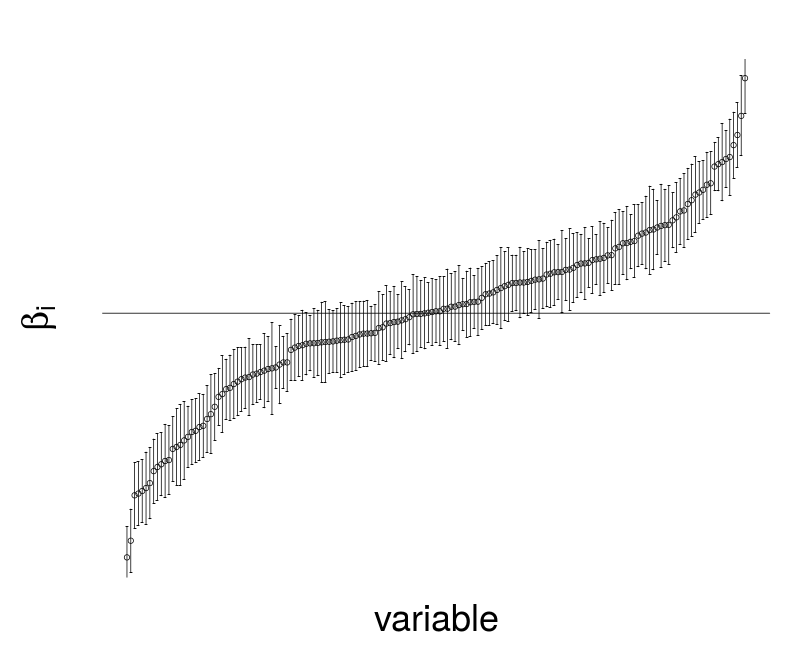
\includegraphics[scale = 0.2]{pf16_coefs.png}
\end{center}
Consider declaring all variables whose intervals cross 0 to be null.
Then $p_1 = 105$ (out of 163)
\end{frame}

\begin{frame}
\frametitle{Example: personality data}
\begin{itemize}
\item If $n$ were large enough, then for the selected model $S$ we
  should have $\hat{y} = \sum_{i=1}^p X\hat{\beta}_i$ close to
  $\hat{y}_S = \sum_{i \in S} X_i \hat{\beta}_i$
\item But...
\end{itemize}
\begin{center}
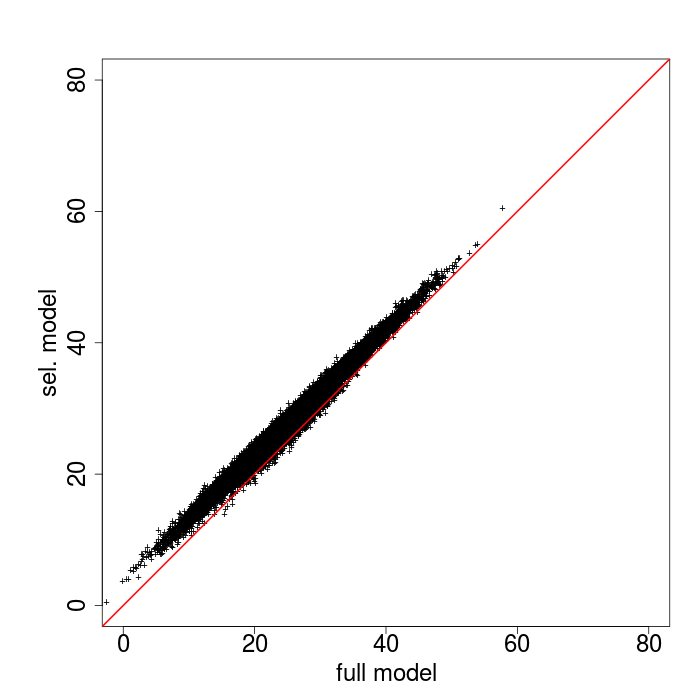
\includegraphics[scale = 0.2]{pf16_modelcheck.png}
\end{center}
\end{frame}

\begin{frame}
\frametitle{Example: personality data}
\begin{itemize}
\item Here $n$ is not large enough for $p = 163$
\item If we reduce the dimensionality to 15 by subsampling columns, it looks more convincing that we selected the correct 10 variables
\end{itemize}
\begin{center}
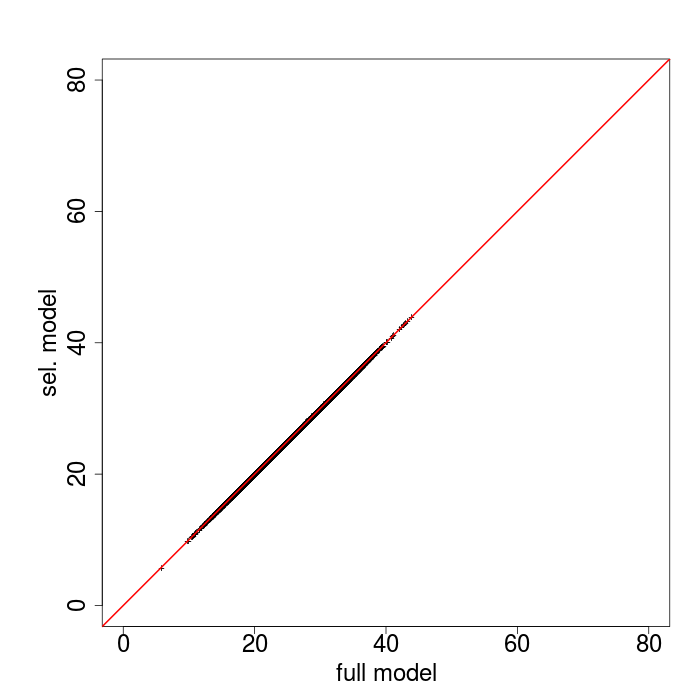
\includegraphics[scale = 0.2]{pf16_modelcheck2.png}
\end{center}
\end{frame}


\begin{frame}
\frametitle{Dillemma}
\begin{itemize}
\item It is by no means \emph{impossible} to get large enough data to estimate high-dimensional $\beta$, with say, $p > 100$
\item But if were \emph{easy} to get such large $n$ data... we wouldn't need these new inference techniques in the first place!
\end{itemize}
\end{frame}

\begin{frame}
\frametitle{Why not use simulations?}
\begin{itemize}
\item<1> Simulations can be used to test robustness of the procedure
\item<1> In simulations, we can add all the nonlinearities, nongaussianity, etc. that we want
\item<2-> Advantage: In simulations, we not only know $\beta$, but exactly how the data is generated
\item<2-> Advantage: We can vary simulation parameters and get a lot of insight about the procedure being tested
\item<3> \textbf{Disadvantage:} Are these simulations relevant?  How can we tell the simulated models are realistic?
\end{itemize}
\end{frame}

\begin{frame}
\frametitle{Idea}
I give you real data \emph{mixed in} with noise variables
\begin{center}
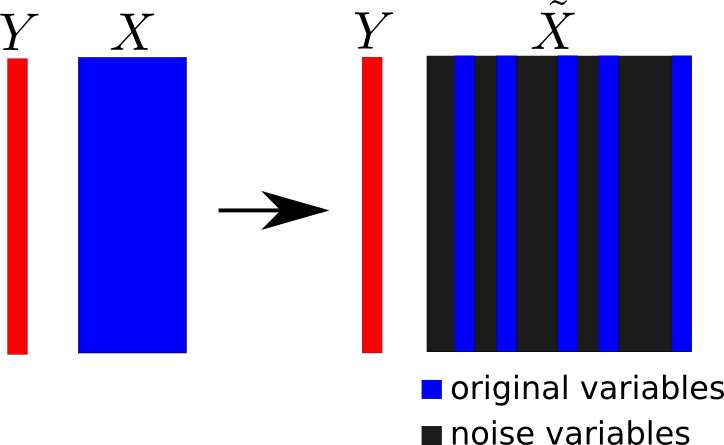
\includegraphics[scale = 0.35]{anc.png}
\end{center}
\begin{itemize}
\item<1-> Can you identify the original columns from the noise columns?
\item<2-> I can test your procedure this way, because I know the ground truth!
\item<3-> \textbf{Caveat}: this test is unrealistically `easy' (due to lack of correlations)
\end{itemize}
\end{frame}

\begin{frame}
\frametitle{Synthetic Negative Controls}
\begin{itemize}
\item Synthetic negative controls (SNCs) are artificial columns \emph{which are correlated} to $X$,
yet still have zero (population) regression coefficients
\item Suppose I give you real data + SNCs, then you apply high-dimensional inference.
If you reject any SNCs, we know these are errors!
\item This gives us some measure of performance on ``real'' data (maybe?)
\end{itemize}
\begin{center}
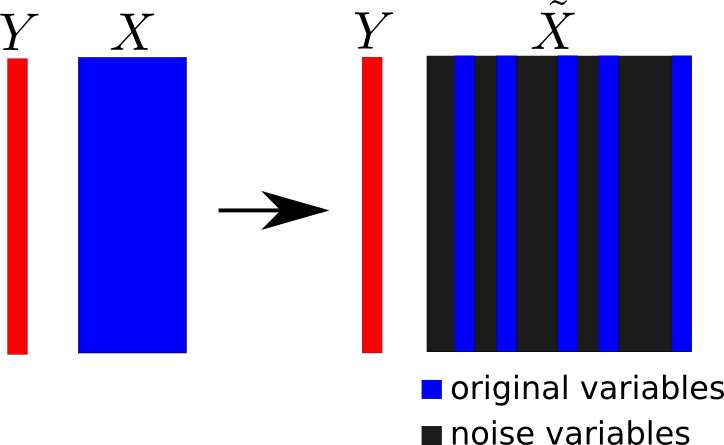
\includegraphics[scale = 0.35]{anc.png}
\end{center}
\end{frame}


\begin{frame}
\frametitle{Synthetic Negative Controls}
\begin{itemize}
\item<1-> Given random vector $x \in \mathbb{R}^p$, let $e$ be noise in $\mathbb{R}^p$ independent of $x$.
\item<1-> Let $\Gamma$ be a fixed $p \times q$ matrix. \emph{Define} synthetic negative controls $z \in \mathbb{R}^{q}$ by
by
\[
z = x'\Gamma + e
\]
and let $\tilde{x} = (x, z)$, so that 
\[
\tilde{x}_1 = x_1,\hdots, \tilde{x}_p = x_p
\]
\[
\tilde{x}_{p+1} = z_1,\hdots, \tilde{x}_{p+q} = z_q
\]
\item<2-> Let
\[
\beta = \E[xx^T]^{-1}\E[yx], \ \ \tilde{\beta} = \E[\tilde{x}\tilde{x}^T]^{-1} \E[y\tilde{x}]
\]
\item<3-> Then
\[
\forall i \in \{1, \hdots, p\}: \beta_i = \tilde{\beta}_i
\]
\[
\forall i \in \{p+1,\hdots, p+q\}: \tilde{\beta}_i = 0
\]
\end{itemize}
\end{frame}

\begin{frame}
\frametitle{Why is this...?}
\begin{itemize}
\item<1> Recall that $\hat{\beta}_i$ is the \emph{univariate regression} coefficient of $Y$
  on $X_{i|-i}$, where $X_{i|-i}$ is the \emph{residual of} $X_i$ after $X_i$ is regressed on the other columns..
\item<1-> Population version: $\beta_i = 0$ if the projection of $X_i$ on the null space of the other covariates is uncorrelated with $Y$
\item<2-3> For $i= 1, \hdots, q$, we have 
\[
\tilde{X}_{p+i} = x' \Gamma_i + E_i
\]
where here $\tilde{X}_{p+1}$ denotes the random variable (not the column of the design matrix)
\item<3-4> The orthogonal projection $P^\perp_X$ of $\tilde{X}_{p+1}$ is
\[
P^\perp_X \tilde{X} = P^\perp_X X \Gamma_i + P^\perp_X E_i = 0 + E_i
\]
since $P^\perp_X X = 0$; meanwhile since $E_i \perp X$, $P^\perp_X E_i = E_i$.
\item<4-5> Since $E_i \perp y$, we have $\text{Cor}(P^\perp_X \tilde{X}_{p+i} , y) = 0$, hence $\tilde{\beta}_{p+i} = 0$
\item<5-> And since $\tilde{\beta}_j = 0$ for all the added variables $j = p+1,\hdots p+q$, it follows that $\tilde{\beta}_i$ is unchanged for $i = 1,\hdots, p$.
\end{itemize}
\end{frame}

\begin{frame}
\frametitle{Using SNCs to evaluate procedures}
\begin{itemize}
\item Take low-dimensional real data mixed with SNCs (synthetic negative controls), apply inference procedure
\item \emph{Proxy for Type I error:} Rejected SNCs
\item \emph{Proxy for Power:} Rejected original variables
\end{itemize}
\end{frame}

\begin{frame}[fragile]
\frametitle{A step-by-step tutorial (in R)}
1. Take the prostate data
\begin{verbatim}
> data(prostate)
> x <- prostate[, 1:8]
> y <- prostate[, 9]
> colnames(x)
[1] "lcavol"  "lweight" "age"     "lbph"    "svi"
    "lcp"     "gleason" "pgg45"  
> dim(x)
[1] 97 8
\end{verbatim}
\end{frame}

\begin{frame}[fragile]
\frametitle{A step-by-step tutorial}
2. Construct 20 synthetic negative controls
\begin{verbatim}
> GAMMA <- matrix(rnorm(8 * 20), 8, 20)
> E <- matrix(rnorm(97 * 20), 97, 20)
> sncs <- as.matrix(x) %*% GAMMA + 2 * E
> sncs <- data.frame(sncs)
> colnames(sncs)
 [1] "X1"  "X2"  "X3"  "X4"  "X5"  "X6" ...
[19] "X19" "X20"
\end{verbatim}
3. Create combined design matrix
\begin{verbatim}
> x2 <- cbind(x, sncs)
\end{verbatim}
\end{frame}

\begin{frame}[fragile]
\frametitle{A step-by-step tutorial}
4. Try marginal screening
\begin{verbatim}
> cors <- cor(x2, y)
> cors[order(-abs(cors)), , drop = F]
              [,1]
lcavol   0.7344603
svi      0.5662182
lcp      0.5488132
X6      -0.4591506
X16      0.4482263
lweight  0.4333194
X4      -0.4326898
\end{verbatim}
\end{frame}

\begin{frame}[fragile]
\frametitle{A step-by-step tutorial}
5. Try covariance test
\begin{verbatim}
> library(covTest)
> covTest(lars(as.matrix(x2), y), as.matrix(x2), y)
$results
 Predictor_Number Drop_in_covariance P-value
                1            69.0292  0.0000
                5             1.5390  0.2219
                2             6.8094  0.0020
               11             0.8559  0.4294
\end{verbatim}
(Numbers 1, 5, 2 are original, 11 is a SNC)
\end{frame}

\begin{frame}[fragile]
\frametitle{A step-by-step tutorial}
6. Try debiased lasso (code at http://web.stanford.edu/~montanar/sslasso/)
\begin{verbatim}
> res <- SSLasso(as.matrix(x2), y)
[1] "10% done"
...
[1] "90% done"
> rej <- (res$up < 0) | (res$low > 0)
> names(x2)[rej]
[1] "lcavol"  "lweight" "svi"    
\end{verbatim}
\end{frame}

\begin{frame}[fragile]
\frametitle{A step-by-step tutorial}
7. Try knockoffs
\begin{verbatim}
> library(knockoff)
> knockoff.filter(x2, y)
Call:
knockoff.filter(X = x2, y = y)

Selected variables:
lweight      X7 
      2      15 
\end{verbatim}
\end{frame}

\begin{frame}
\frametitle{Disclaimer!}
\begin{itemize}
\item I am \emph{not} proposing SNCs as a methodology for \emph{inference}
\item There is a danger of inferring \emph{that Type I error has been controlled} from lack of rejection of SNCs.
There are no formal guarantees of this!
\item One should interpret results from experiments with SNCs in the same way one interprets simulation results with purely synthetic data
\end{itemize}
\end{frame}

\begin{frame}
\frametitle{More Experiments!}
\begin{center}
\begin{tabular}{|c|c|c|c|c|c|}
\hline
Data & $n$ & $p_1$ & Linear? & Gaussian? & Constant $\sigma^2$?\\ \hline
Personality & 3000 & 163 & No & No & No\\ \hline
fMRI & 1750 & 53 & No & OK & No \\ \hline
HIV & 842 & 207 & No & Yes? & OK? \\ \hline
Galaxy & 323 & 4 & No & OK & No \\ \hline
\end{tabular}
\end{center}
\begin{itemize}
\item We add $n/2 - p_1$ synthetic negative controls
\item $X$ is scaled, $\Gamma$ is a gaussian matrix, $Var(E)$ is chosen to yield `interesting' results
\item Personality data is subsampled
\end{itemize}
\end{frame}

\begin{frame}
\frametitle{Marginal Screening}

\begin{center}
\begin{tabular}{cc}
Personality & fMRI \\
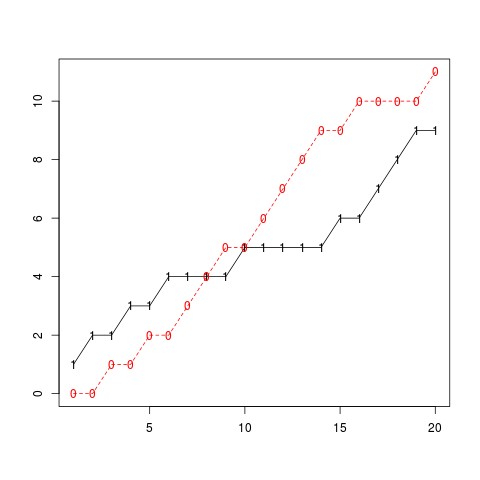
\includegraphics[scale=0.15]{mar_pf16.png} & 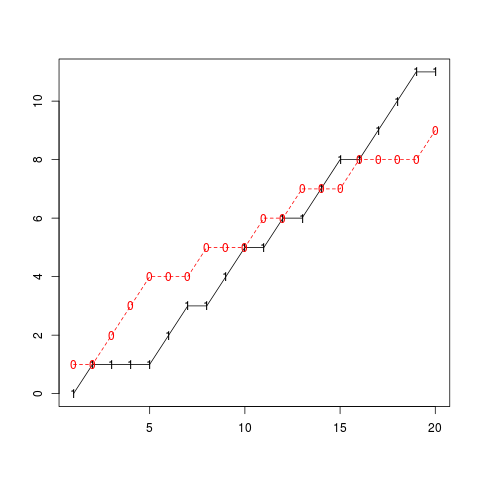
\includegraphics[scale=0.15]{mar_fMRI.png}\\
HIV & Galaxy\\
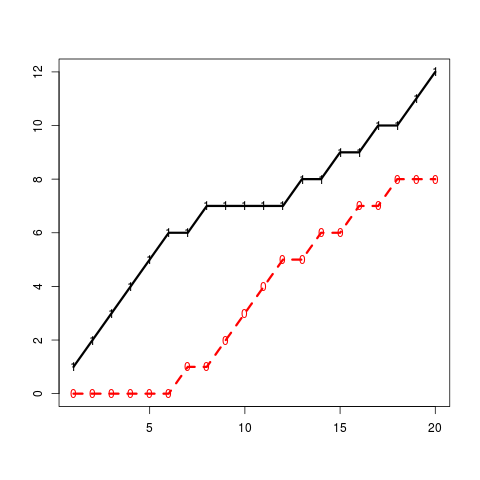
\includegraphics[scale=0.15]{mar_HIV.png} & 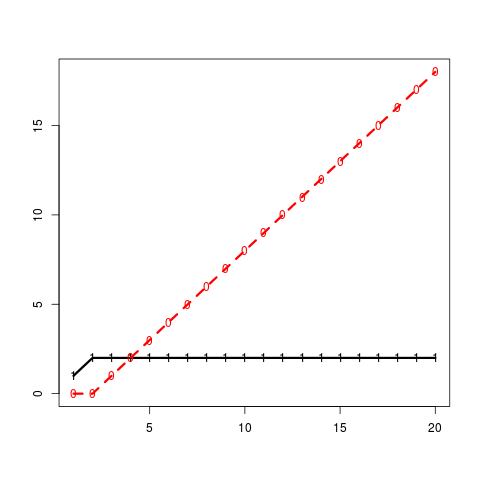
\includegraphics[scale=0.15]{mar_gal.png}\\
\end{tabular}

Legend: \textcolor{red}{0} = False positives, 1 = True positives
\end{center}
\end{frame}

\begin{frame}
\frametitle{Ordinary Least Squares}
``Rel. power" =  TP/(max number of TPs  at $\alpha = 0.5$ for any method)

\begin{center}
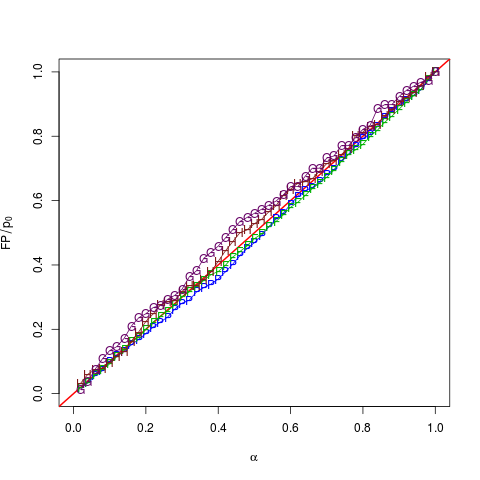
\includegraphics[scale = 0.3]{res_o_type1.png}
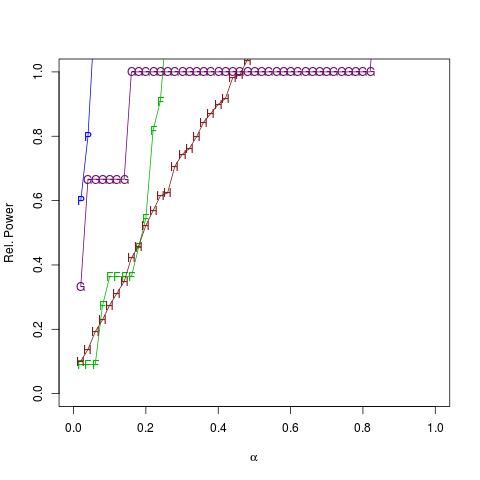
\includegraphics[scale = 0.3]{res_o_power.png}
\end{center}

Legend: \textcolor{blue}{P} = Personality, \textcolor{green}{F} = fMRI,
\textcolor{red}{H} = HIV, \textcolor{violet}{G} = Galaxy
\end{frame}

\begin{frame}
\frametitle{Debiased Lasso}
Can you spot the difference from the previous slide?

\begin{center}
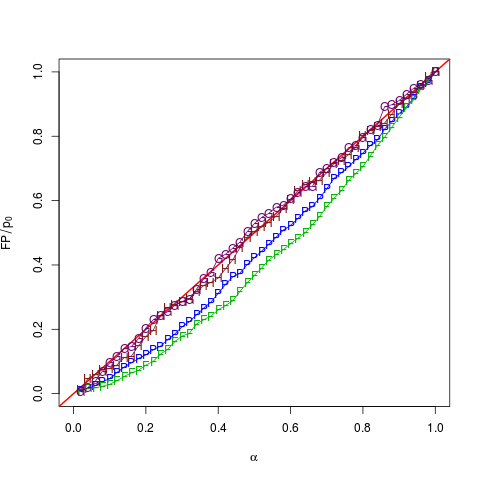
\includegraphics[scale = 0.3]{res_s_type1.png}
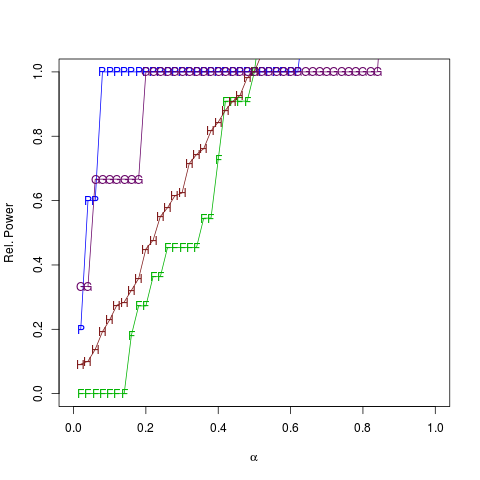
\includegraphics[scale = 0.3]{res_s_power.png}
\end{center}

Legend: \textcolor{blue}{P} = Personality, \textcolor{green}{F} = fMRI,
\textcolor{red}{H} = HIV, \textcolor{violet}{G} = Galaxy
\end{frame}



\begin{frame}
\frametitle{Covariance Test}
\emph{Forward Stop:} reject first $\hat{k}$, where $-\frac{1}{\hat{k}}\sum_{i=1}^{\hat{k}} \log(1-p_i) \leq \alpha$

\begin{center}
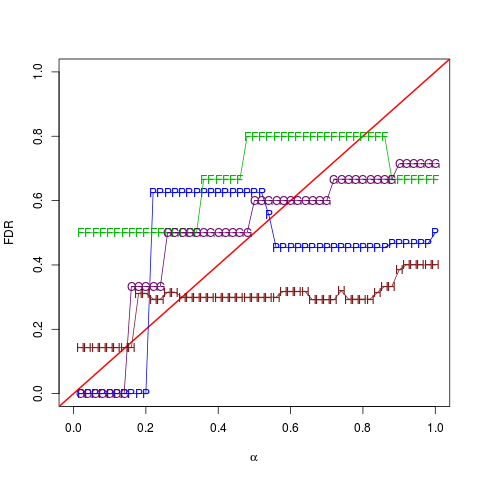
\includegraphics[scale = 0.3]{res_c_fs_type1.png}
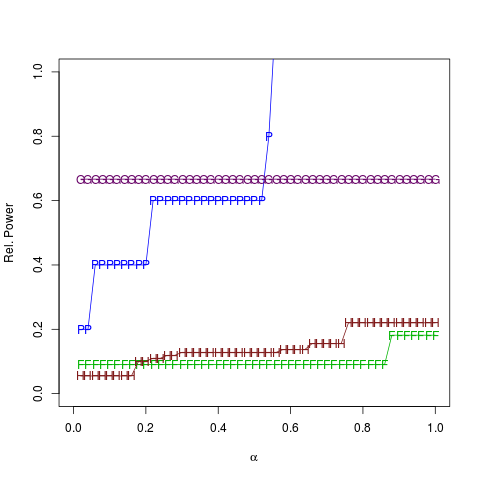
\includegraphics[scale = 0.3]{res_c_fs_power.png}
\end{center}

Legend: \textcolor{blue}{P} = Personality, \textcolor{green}{F} = fMRI,
\textcolor{red}{H} = HIV, \textcolor{violet}{G} = Galaxy
\end{frame}

\begin{frame}
\frametitle{Covariance Test}
\emph{Strong Stop:} reject first $\hat{k}$, where $\frac{m}{\hat{k}}e^{\sum_{j=\hat{k}}^{p} \log(p_j)/j} \leq \alpha$

\begin{center}
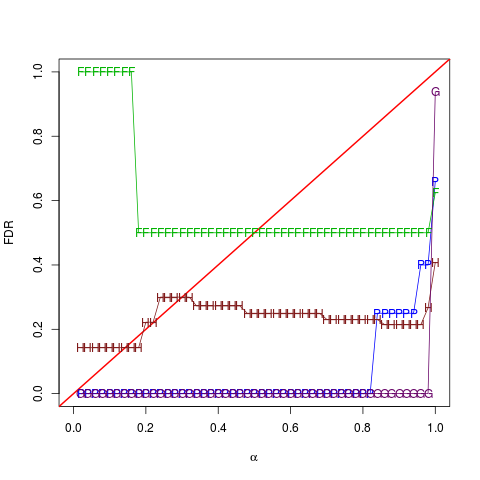
\includegraphics[scale = 0.3]{res_c_ss_type1.png}
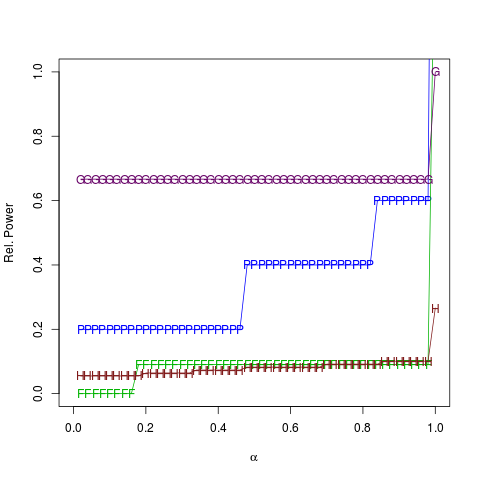
\includegraphics[scale = 0.3]{res_c_ss_power.png}
\end{center}

Legend: \textcolor{blue}{P} = Personality, \textcolor{green}{F} = fMRI,
\textcolor{red}{H} = HIV, \textcolor{violet}{G} = Galaxy
\end{frame}

\begin{frame}
\frametitle{Knockoffs}
Using Knockoff+ threshhold

\begin{center}
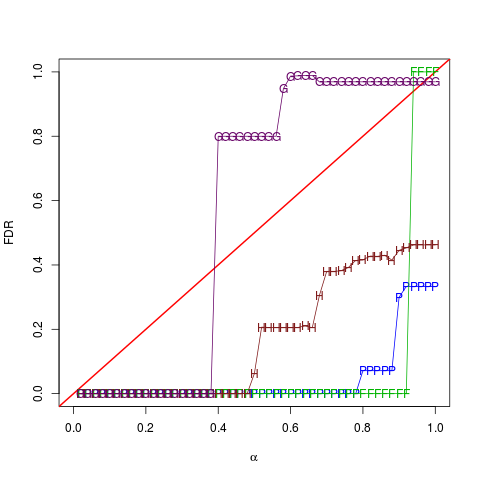
\includegraphics[scale = 0.3]{res_kp_type1.png}
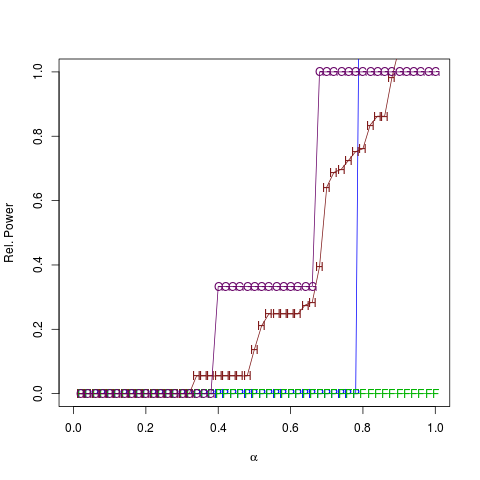
\includegraphics[scale = 0.3]{res_kp_power.png}
\end{center}

Legend: \textcolor{blue}{P} = Personality, \textcolor{green}{F} = fMRI,
\textcolor{red}{H} = HIV, \textcolor{violet}{G} = Galaxy
\end{frame}


\begin{frame}
\frametitle{Knockoffs}
\emph{Note:} $FDR^* = \E[FP/(FP + TP + 1/\alpha)]$

\begin{center}
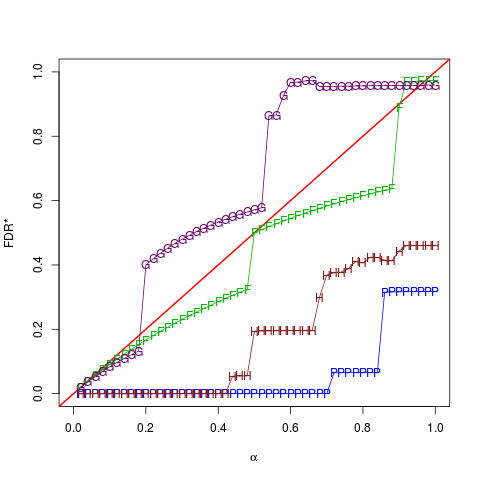
\includegraphics[scale = 0.3]{res_k_type1.png}
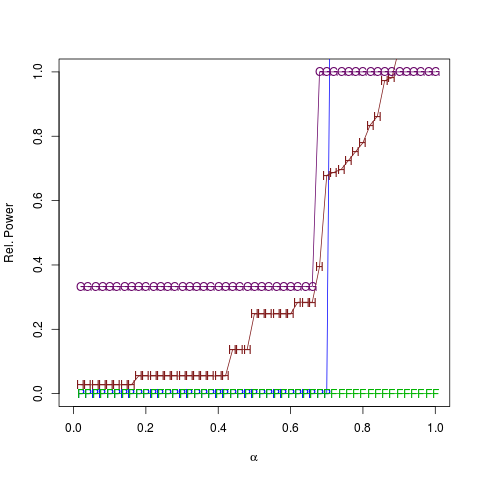
\includegraphics[scale = 0.3]{res_k_power.png}
\end{center}

Legend: \textcolor{blue}{P} = Personality, \textcolor{green}{F} = fMRI,
\textcolor{red}{H} = HIV, \textcolor{violet}{G} = Galaxy
\end{frame}


\begin{frame}
\frametitle{Variable Ranking Criteria}
\begin{itemize}
\item Forget about Type I error for a second... 
\item Use procedures to \emph{rank} variables by p-value
\item Easy to compare procedures with different Type I criteria and also non-inference variable selection
\item (Optional) score by Area Under Curve (AUC), etc.
\end{itemize}
\end{frame}

\begin{frame}
\frametitle{Variable Ranking: Personality}
\begin{center}
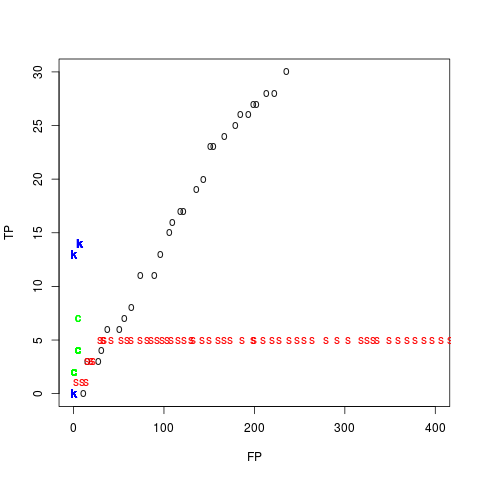
\includegraphics[scale = 0.35]{pf16_tvf.png}
\end{center}

Legend: o = OLS, \textcolor{green}{c} = covariance test,
\textcolor{blue}{k} = knockoff, \textcolor{red}{s} = debiased lasso,
(line) = marginal screening, \textcolor{green}{(line)} = lasso path
\end{frame}

\begin{frame}
\frametitle{Variable Ranking: fMRI}
\begin{center}
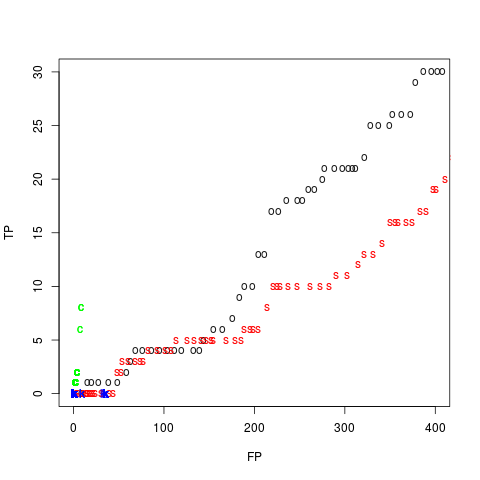
\includegraphics[scale = 0.35]{fMRI_tvf.png}
\end{center}

Legend: o = OLS, \textcolor{green}{c} = covariance test,
\textcolor{blue}{k} = knockoff, \textcolor{red}{s} = debiased lasso,
(line) = marginal screening, \textcolor{green}{(line)} = lasso path
\end{frame}

\begin{frame}
\frametitle{Variable Ranking: HIV}
\begin{center}
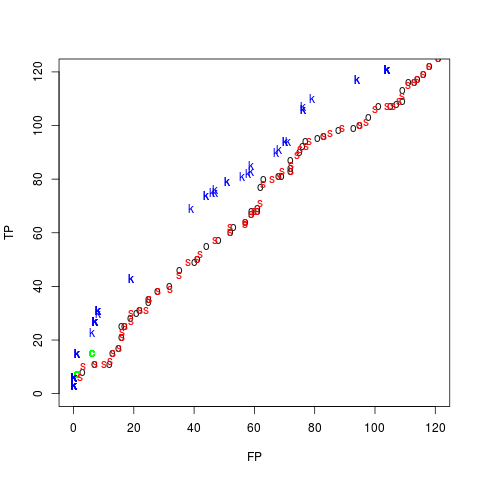
\includegraphics[scale = 0.35]{HIV_tvf.png}
\end{center}

Legend: o = OLS, \textcolor{green}{c} = covariance test,
\textcolor{blue}{k} = knockoff, \textcolor{red}{s} = debiased lasso,
(line) = marginal screening, \textcolor{green}{(line)} = lasso path
\end{frame}

\begin{frame}
\frametitle{Variable Ranking: Galaxy}
\begin{center}
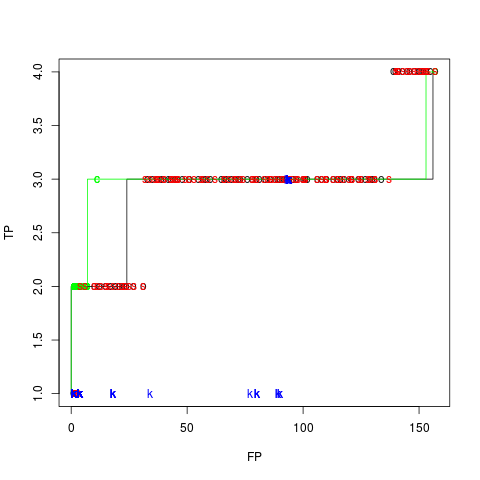
\includegraphics[scale = 0.35]{gal_tvf.png}
\end{center}

Legend: o = OLS, \textcolor{green}{c} = covariance test,
\textcolor{blue}{k} = knockoff, \textcolor{red}{s} = debiased lasso,
(line) = marginal screening, \textcolor{green}{(line)} = lasso path
\end{frame}


\begin{frame}
\frametitle{Commentary}
\begin{itemize}
\item We should not conclude too much from four experiments with rather arbitrary generation parameters...
\item Debiased lasso similiar to OLS but more conservative, less powerful
\item Knockoffs vs covariance test:
\begin{itemize}
\item Knockoffs may control FDR more robustly than Covariance test (especially at small $\alpha$)
\item Knockoffs and covariance are similar in power overall but have different case-by-case behavior
\end{itemize}
\item Knockoffs tend to be conservative, but have good variable ranking in some cases (Personality, fMRI)
\item Marginal screening remains annoyingly effective...
\end{itemize}
\end{frame}

\begin{frame}
\frametitle{Another look at covTest}
 \begin{columns}[c]
    \column{.5\textwidth}
     \emph{Strong stop type I error}

     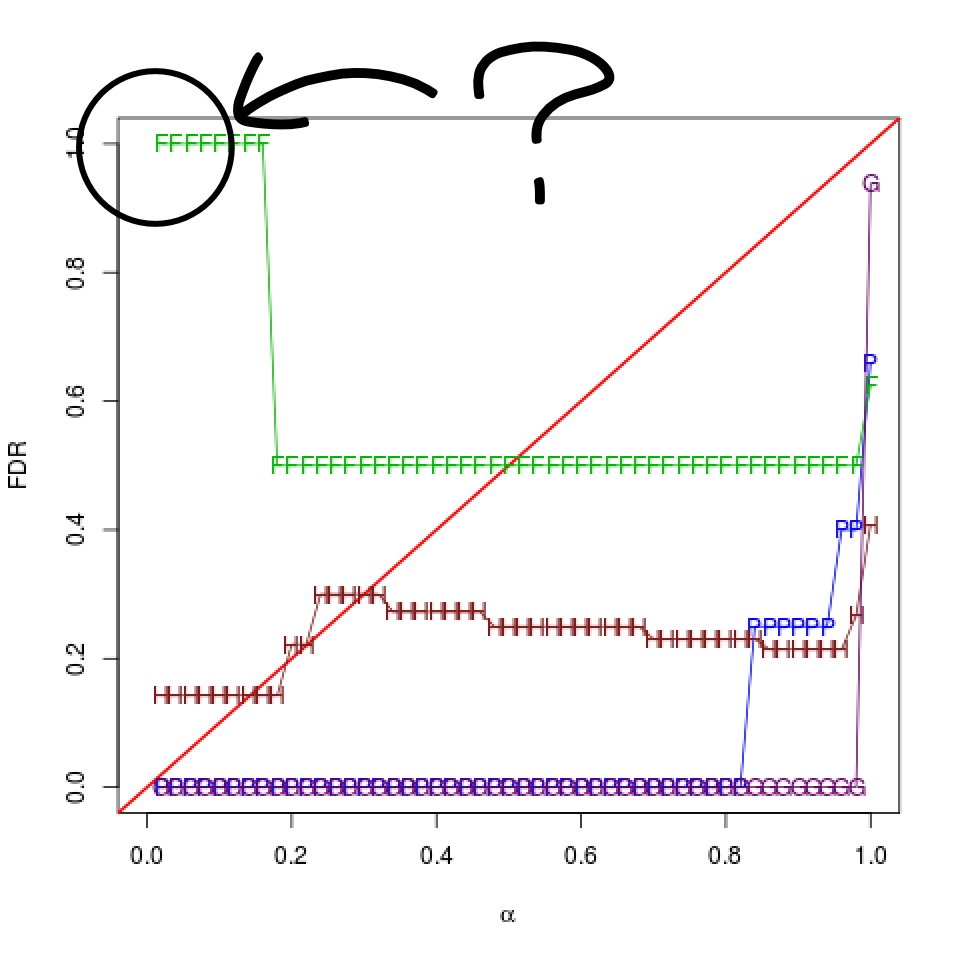
\includegraphics[scale = 0.4]{res_c_ss_type1_comment.png}
    \column{.5\textwidth}
     \begin{itemize}
       \item<1> Why did this negative control get rejected in the fMRI data at such a low $\alpha$?
       \item<2> According to the \emph{incremental null}, the negative control was not a mistake... it is the best single predictor by far!
       \item<2> The particular negative control took an \emph{average} of the original columns 
       \item<3> It is true that $\beta_i = 0$ for the rejected variable... but should we really disregard such strong "proxy'' variables?
     \end{itemize}
 \end{columns}
(thanks to Stefan!)
\end{frame}

\begin{frame}
\frametitle{Low sample size}
\begin{center}
\begin{tabular}{|c|c|c|c|c|c|c|}
\hline
Data & $n$ & $p$ & $p_1$ & Linear? & Gaussian? & Constant $\sigma^2$?\\ \hline
Personality & 100 & 1500 & 163 & No & No & No\\ \hline
fMRI & 100 & 875 & 53 & No & OK & No \\ \hline
HIV & 100 & 421 & 207 & No & Yes? & OK? \\ \hline
Galaxy & 100 & 161 & 4 & No & OK & No \\ \hline
\end{tabular}
\end{center}
\begin{itemize}
\item Reduce the sample size to 100, so that $p >> n$
\item Same number of negative controls, but larger added noise (easier)
\item Covariance test requires estimate $\hat{\sigma}$: ``cheat'' by using OLS estimate from \emph{original} data
\end{itemize}
\end{frame}


\begin{frame}
\frametitle{Debiased Lasso}

\begin{center}
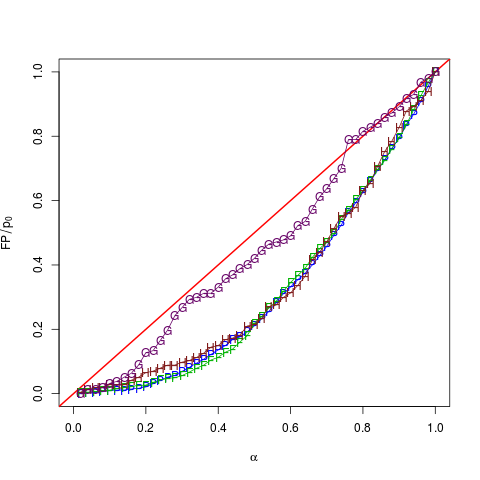
\includegraphics[scale = 0.3]{ress_s_type1.png}
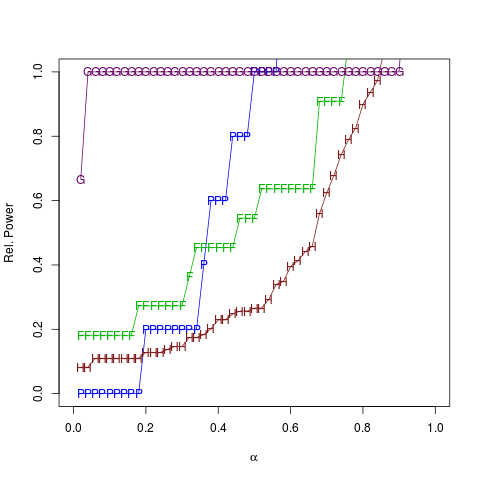
\includegraphics[scale = 0.3]{ress_s_power.png}
\end{center}

Legend: \textcolor{blue}{P} = Personality, \textcolor{green}{F} = fMRI,
\textcolor{red}{H} = HIV, \textcolor{violet}{G} = Galaxy
\end{frame}


\begin{frame}
\frametitle{Covariance Test}
\emph{Forward Stop:} reject first $\hat{k}$, where $-\frac{1}{\hat{k}}\sum_{i=1}^{\hat{k}} \log(1-p_i) \leq \alpha$

\begin{center}
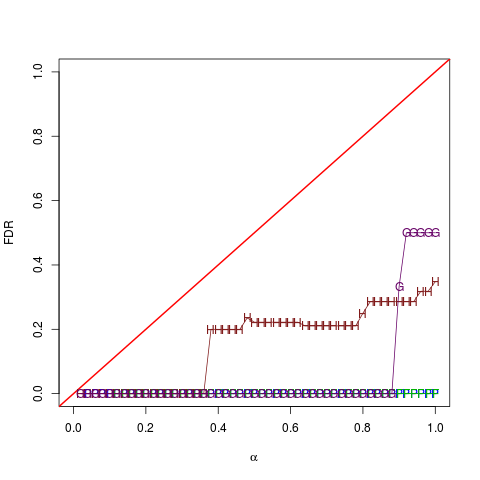
\includegraphics[scale = 0.3]{ress_c_fs_type1.png}
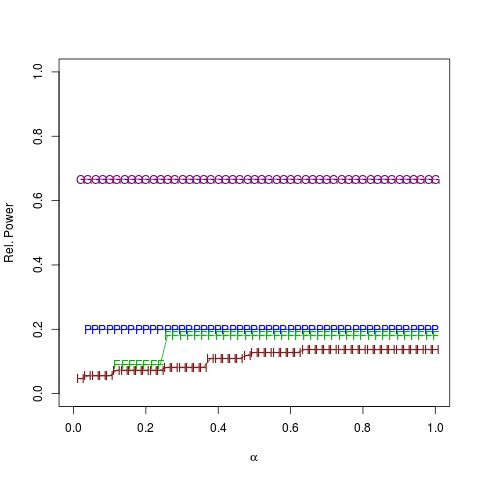
\includegraphics[scale = 0.3]{ress_c_fs_power.png}
\end{center}

Legend: \textcolor{blue}{P} = Personality, \textcolor{green}{F} = fMRI,
\textcolor{red}{H} = HIV, \textcolor{violet}{G} = Galaxy
\end{frame}

\begin{frame}
\frametitle{Covariance Test}
\emph{Strong Stop:} reject first $\hat{k}$, where $\frac{m}{\hat{k}}e^{\sum_{j=\hat{k}}^{p} \log(p_j)/j} \leq \alpha$

\begin{center}
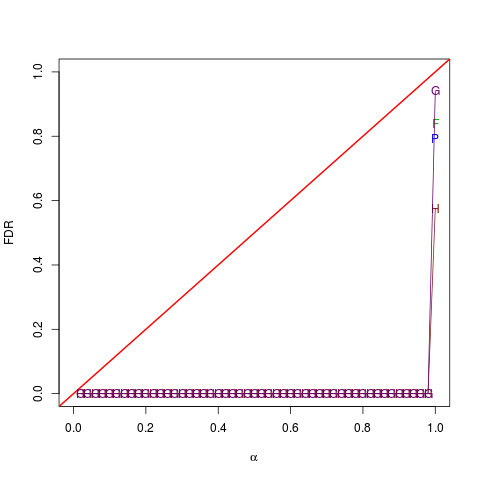
\includegraphics[scale = 0.3]{ress_c_ss_type1.png}
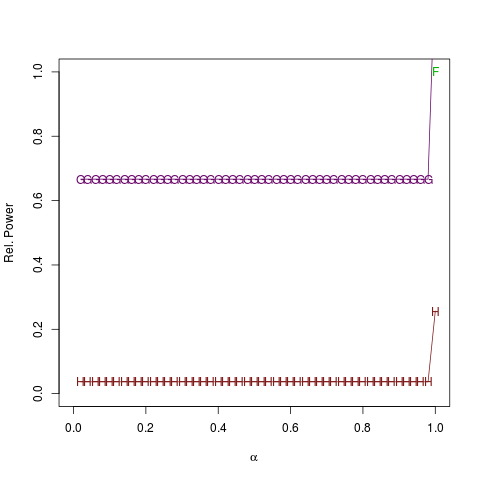
\includegraphics[scale = 0.3]{ress_c_ss_power.png}
\end{center}

Legend: \textcolor{blue}{P} = Personality, \textcolor{green}{F} = fMRI,
\textcolor{red}{H} = HIV, \textcolor{violet}{G} = Galaxy
\end{frame}

\begin{frame}
\frametitle{Commentary}
\begin{itemize}
\item Debiased lasso and Covariance test + forward stop continue to control Type I error while finding true positives
\item Covariance test + strong stop appears too conservative
\end{itemize}
\end{frame}


\begin{frame}
\frametitle{Can we really trust these experiments!?}
\begin{itemize}
\item<1-> Here we are implicitly assuming that real data always consists of a few ``active variables'' and many null variables
\item<1-> If that's true, it seems reasonable to model the distribution of the inactive variables conditional on knowing a superset of the active variables
\item<2-> But how do we know that $\beta$ is really sparse?
\item<2-> Even more importantly, how do we know that inferring coefficients of the
  \emph{full model} $\beta$ are a meaningful objective?  E.g. should we consider the
  covariance test to have made a mistake in the fMRI data?
\item<3-> How can we decide between the \emph{full model null}, the
  \emph{incremental null}, or an entirely different framework
  altogether?
\item<3-> \emph{Feedback from the practitioner} is the only way we can
  tell if we have the right formulation for any particular application
\end{itemize}
\end{frame}

\begin{frame}
\frametitle{Questions to consider}
\begin{itemize}
\item Why is OLS more powerful than lasso in some of these experiments even when $\beta$ is sparse? Look at covariance conditions in the theory of LASSO...
\item Why do knockoffs or lasso beat marginal screening/OLS in the HIV data? Was it due to how we generated the SNCs or is due to something special about the data itself?
\item Suppose we wanted to validate selective inference or the incremental null.  How can we do this with synthetic negative controls (other than pure noise?)
\end{itemize}
\end{frame}

\begin{frame}
\frametitle{Closing thoughts}
\begin{quotation}
`` Both the client and the statistician... must base their thinking on
  a recognition that their assumptions will always require review and
  reappraisal...  ''
\end{quotation}
\hfill -- John Tukey
\end{frame}

\begin{frame}
\frametitle{Acknowledgements}
Thanks to Will Fithian and Stefan Wager for useful discussions.
\end{frame}

\begin{frame}
\frametitle{References}
\begin{itemize}
\item Barber, R., and Candes, E. (2014). Controlling the False Discovery Rate via Knockoffs. arXiv Preprint arXiv:1404.5609, 1–27. Retrieved from http://arxiv.org/abs/1404.5609
\item G’Sell, Max Grazier. Wager, Stefan
Chouldechova, Alexandra.
Tibshirani, Robert. “Sequential Selection Procedures and False Discovery Rate Control.” (2013): 31. Web. 7 May 2015.
\item Javanmard, A., and Montanari, A. (2014). Confidence intervals and hypothesis testing for high-dimensional regression. The Journal of Machine Learning Research, 15, 2869–2909. Retrieved from http://dl.acm.org/citation.cfm?id=2697057
\item Lockhart, R., Taylor, J., Tibshirani, R. J., and Tibshirani, R. (2014). a Significance Test for the Lasso. Annals of Statistics, 42(2), 413–468. doi:10.1214/13-AOS1175
\end{itemize}
\end{frame}



\end{document}








\[
X = [1 | X_1 | \hdots | X_p] = \begin{pmatrix}x_1^T \\ \vdots \\ x_n^T \end{pmatrix}, \ \ Y = \begin{pmatrix}y_1 \\ \vdots \\ y_n \end{pmatrix}
\]
and
\[
\tilde{X} =  [X | X_{p+1} | \hdots | X_{p+1}] = 
\begin{pmatrix}\tilde{x}_1^T \\ \vdots \\ \tilde{x}_n^T \end{pmatrix}
\]
Let


\begin{frame}
\frametitle{What are we learning?}
\begin{itemize}
\item<1-> \emph{Claim:} Performance on data with \emph{known active variables} + SNCs are informative of how inference procedures generally perform in similar data with \emph{unknown active variables}
\item<2-> Example (GWAS): There is a new disease (say, liver cancer) where we have little prior info.  I have data for a `similar' disease, (say, stomach cancer) for which I have \emph{partial information} about the relevant causes. In particular, I know \emph{the most important} the genes involved stomach cancer
\item<2-> Testing your procedure directly on the stomach cancer data is uninformative: if you reject a gene which is not \emph{a priori} known to cause stomach cancer... it could still be a new discovery! 
\item<3-> Rather than test your inference procedure on the full stomach cancer data, test it on the subset of the \emph{known genes} plus SNCs
\item<3-> Tricky part: choosing the size of the noise for the SNCs.  To be safe, try several noise levels.
\end{itemize}
\end{frame}

\begin{frame}
\frametitle{How could this be useful?}
\begin{itemize}
\item<1-> There are no formal guarantees... so what could we gain from using SNC experiments?
\item<2-> We can complement \emph{theoretical guarantees} with \emph{application-specific benchmarks}
\item<3-> Poor performance on benchmarks would tell us where our methods need improvement
\begin{itemize}
\item Failure to control Type I error on benchmarks indicates a need for methods derived under weaker assumptions
\item Overly conservative Type I error control indicates a need for methods which are more adaptive to `easy' cases
\end{itemize}
\item<4-> Possible to run a Kaggle-style competition for \emph{inference} rather than prediction
\item<5-> Recognizing that different procedures can have differing strengths creates room for a diversity of approaches
\end{itemize}
\end{frame}


\begin{frame}
\frametitle{Covariance Test}
\emph{Naive procedure:} continue rejecting until $p > \alpha$, then accept all other variables

\begin{center}
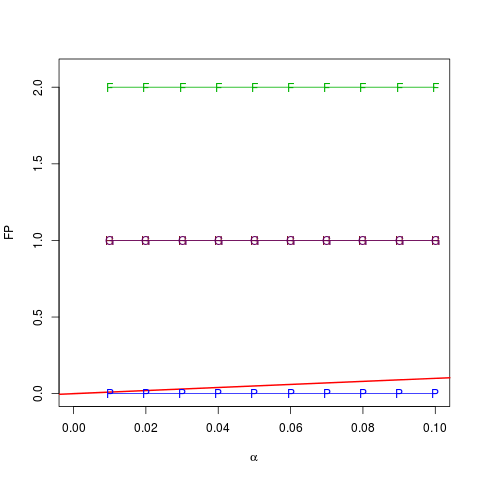
\includegraphics[scale = 0.3]{res_c_type1.png}
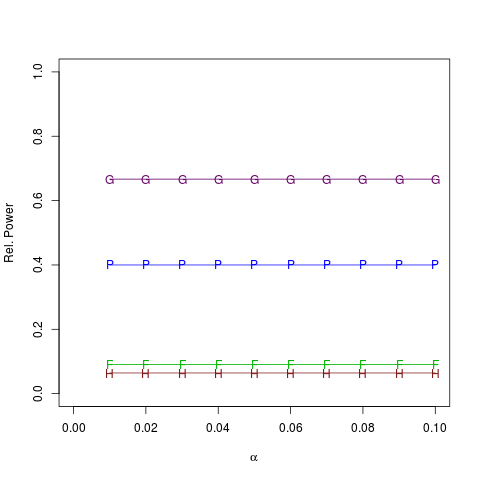
\includegraphics[scale = 0.3]{res_c_power.png}
\end{center}

Legend: \textcolor{blue}{P} = Personality, \textcolor{green}{F} = fMRI,
\textcolor{red}{H} = HIV, \textcolor{violet}{G} = Galaxy
\end{frame}
